\documentclass[openany,zihao=-4,UTF8]{ctexart}
\usepackage[a4paper,margin=2.5cm]{geometry}
\usepackage{amsmath}                                    % 排版数学公式

% 使equation计数器也依赖于section计数器
\numberwithin{equation}{section}

% 使table计数器也依赖于section计数器
\numberwithin{table}{section}

% 使figure计数器也依赖于section计数器
\numberwithin{figure}{section}

\usepackage{latexsym}
\usepackage{amsfonts}                                   %数学符号字体库宏包套件,它包含有:amsfonts、amssymb、eufrak 和 eucal 四个宏包。
\usepackage{amssymb}                                    % 定义AMS的数学符号命令
\usepackage{mathrsfs}                                   % 数学RSFS书写字体
\usepackage{bm}                                         % 数学黑体
\usepackage{graphicx}                                   % 支持插图,图形宏包graphics的扩展宏包
\usepackage{color,xcolor}                               % 支持彩色
\usepackage{amscd}
\usepackage[linesnumbered,ruled,vlined]{algorithm2e}
\usepackage{diagbox}
\usepackage{minted}
\usepackage{titlesec}                                   %设置章节格式
\usepackage{tcolorbox}

% 设置 paragraph 为只有一级编号(从1开始)
\renewcommand{\theparagraph}{\arabic{paragraph}} % 只显示一级编号
\makeatletter
\@addtoreset{paragraph}{section} % 每节开始时重置 paragraph 计数器
\makeatother

%%文本框设置
\newcommand{\tbox}[1]{
  \begin{center}
    \begin{tcolorbox}[colback=gray!10,%gray background
        colframe=black,% black frame colour
        width=14cm,% Use 8cm total width,
        arc=1mm, auto outer arc,
        boxrule=0.5pt,
      ]
      {#1}
    \end{tcolorbox}
  \end{center}
}

% 设置 paragraph 为 block 风格,自动换行
\titleformat{\paragraph}[block]
  {\normalfont\normalsize\bfseries}{\theparagraph.}{0.5em}{}

% 设置标题后换行(after-sep 设为 \newline)
\titlespacing*{\paragraph}{0pt}{3.25ex plus 1ex minus .2ex}{0pt}
  
\usepackage{enumerate}                                 	%更改enumerate环境格式
\usepackage{hyperref}

%改变超链接颜色
\hypersetup{
    colorlinks=true,
    linkcolor=blue,
    filecolor=blue,      
    urlcolor=blue,
    citecolor=cyan,
}

\usepackage{subcaption}
\usepackage{minipage-marginpar}
\usepackage{float}%提供float浮动环境
\usepackage{booktabs}%提供命令\toprule、\midrule、\bottomrule
\usepackage{listings}
\usepackage{xcolor}
\usepackage{tabularx}
\usepackage{multirow}
\usepackage[perpage]{footmisc}

% 自定义命令,用于角标引用文献和交叉引用
\newcommand{\scite}[1]{\textsuperscript{\cite{#1}}}
\newcommand{\sref}[1]{\textsuperscript{\ref{#1}}}
\newcommand{\bs}[1]{\boldsymbol{#1}}
\newcommand{\romannumber}[1]{\uppercase\expandafter{\romannumeral#1}}
\newcommand{\alert}[1]{\textcolor{red}{#1}}
%%对一些autoref的中文引用名作修改
\def\equationautorefname{式}
\def\footnoteautorefname{脚注}
\def\itemautorefname{项}
\def\figureautorefname{图}
\def\tableautorefname{表}
\def\partautorefname{篇}
\def\appendixautorefname{附录}
\def\chapterautorefname{章}
\def\sectionautorefname{节}
\def\subsectionautorefname{小小节}
\def\subsubsectionautorefname{subsubsection}
\def\paragraphautorefname{段落}
\def\subparagraphautorefname{子段落}
\def\FancyVerbLineautorefname{行}
\def\theoremautorefname{定理}

% 设置标题层级和目录层级
\setcounter{tocdepth}{3}
\setcounter{secnumdepth}{4}
\usepackage{rotating}

% ----------------------------
% 代码显示相关宏包
% ----------------------------
\usepackage{listings}     % 代码高亮

% ----------------------------
% 设置代码样式
% ----------------------------
\definecolor{codegray}{rgb}{0.5,0.5,0.5}
\definecolor{backcolor}{rgb}{0.95,0.95,0.95}
\definecolor{codeblue}{rgb}{0.2,0.2,0.6}
\definecolor{keywordcolor}{rgb}{0.1,0.1,0.6}
\definecolor{stringcolor}{rgb}{0.58,0,0.1}

\lstdefinestyle{pythonstyle}{
    backgroundcolor=\color{backcolor},   
    commentstyle=\color{codegray}\itshape,
    keywordstyle=\color{keywordcolor}\bfseries,
    stringstyle=\color{stringcolor},
    numberstyle=\tiny\color{gray},
    basicstyle=\ttfamily\footnotesize,
    breaklines=true,                     
    captionpos=b,                        
    keepspaces=true,
    numbers=left,                        
    numbersep=5pt,                       
    showspaces=false,                    
    showstringspaces=false,
    showtabs=false,                      
    tabsize=4,
    language=Python
}

% 设置默认样式
\lstset{style=pythonstyle}

\title{程序说明}
\author{欧阳嘉鸿}
\date{\today}
\begin{document}
\maketitle
\newpage
\tableofcontents
\newpage
\section{探测任务规划问题建模}
本问题旨在为多个地面雷达调度多个空间目标的观测任务,实现有效资源分配并最大化任务完成度。

\subsection{决策变量}
定义如下布尔型决策变量:
$$
    x_{r,s,a} =
    \begin{cases}
        1, & \text{若雷达 } r \text{ 在其第 } a \text{ 个可见弧段对目标 } s \text{ 进行观测} \\
        0, & \text{否则}
    \end{cases}
$$
其中:$r \in R$(雷达集合),$s \in S$(目标集合),$a \in A_{r,s}$(雷达 $r$ 对目标 $s$ 可观测的弧段索引集合)

此外,引入辅助二值变量 $y_s$ 表示目标 $s$ 是否被有效观测:
$$
    y_s =
    \begin{cases}
        1, & \text{若目标 } s \text{ 满足所有观测需求约束} \\
        0, & \text{否则}
    \end{cases}
$$

\subsection{目标函数}
目标函数为最大化加权有效观测目标数:
$$
    \max J = \sum_{s \in S} w_s \cdot y_s
$$
其中:
\begin{itemize}
    \item $w_s$:目标 $s$ 的权重(优先级);
    \item $y_s$:二值变量,表示目标 $s$ 是否为有效观测目标。
\end{itemize}

\subsection{约束条件}
\subsubsection{雷达观测容量约束}
每部雷达在任一时刻最多只能同时观测 $C_r$ 个目标。考虑离散时间索引 $t \in T$,有:
$$
    \sum_{s \in S} \sum_{a \in A_{r,s}^t} x_{r,s,a} \leq C_r, \quad \forall r \in R,\ \forall t \in T
$$
其中:
\begin{itemize}
    \item $A_{r,s}^t$:时刻 $t$ 时,雷达 $r$ 可用于观测目标 $s$ 的弧段集合;
    \item $T$:时间步长集合。
\end{itemize}

\subsubsection{单次观测时长约束}
对于每个弧段 $(r, s, a)$,如果其持续时间小于目标 $s$ 所需的最小观测时间 $T_s^{\min}$,则禁止使用该弧段:
$$
    x_{r,s,a} = 0, \quad \text{if } \Delta t_{r,s,a} < T_s^{\min}
$$
其中 $\Delta t_{r,s,a}$ 是弧段 $(r, s, a)$ 的持续时间。

\subsubsection{目标有效性判定约束}
利用中间变量辅助建模,通过观测决策 $x_{r,s,a}$ 与弧段持续时间 $\Delta t_{r,s,a}$ 的乘积累加可得目标有效观测时长,再结合目标对观测数量和测站的要求,判定 $y_s$。

1. 统计目标 $s$ 被多少个不同的雷达观测过:
$$
    O_r(s) = \sum_{a \in A_{r,s}} x_{r,s,a}, \quad \forall r \in R,\ s \in S
$$
其中 $O_r(s)$ 表示雷达 $r$ 对目标 $s$ 的有效观测次数。

2. 统计雷达数量:
$$
    N_r(s) = \sum_{r \in R} z_{r,s}, \quad \text{where } z_{r,s} = 
    \begin{cases}
        1, & \text{if } O_r(s) \geq 1 \\
        0, & \text{otherwise}
    \end{cases}
$$
其中 $z_{r,s}$ 是一个辅助二值变量,表示雷达 $r$ 是否对目标 $s$ 有过有效观测。

3. 判断目标是否为有效观测目标:
$$
    y_s = 
    \begin{cases}
        1, & \text{if } N_r(s) = M_s^{\min} \text{ and } \sum_{r \in R} \sum_{a \in A_{r,s}} x_{r,s,a} = N_s^{\min} \\
        0, & \text{otherwise}
    \end{cases}
$$
其中:
\begin{itemize}
    \item $M_s^{\min}$:目标 $s$ 所需的最小观测测站数;
    \item $N_s^{\min}$:目标 $s$ 所需的最小有效观测次数。
\end{itemize}

\subsection{可见弧段预处理与切割策略}
为了更精细地调度雷达观测资源,在模型构建前对原始可见弧段进行了切割处理。由于某些长持续时间的可见弧段可能包含多个可独立使用的子弧段,我们采用滑动窗口重叠切割方法(Overlap-based Sliding Window Splitting),将每个原始弧段划分为若干个等长度的小弧段,其持续时间等于目标所需的最小观测时间 $T_s^{\min}$,并保留一定比例的重叠以提升调度灵活性。

具体实现如下:  
对于任意一个原始弧段 $(t_{\text{start}}, t_{\text{end}}, \Delta t)$,若其总时长大于或等于该目标所需最小观测时间 $T_s^{\min}$,则使用步长为 $T_s^{\min} \cdot (1 - \texttt{overlap\_ratio})$ 的滑动窗口进行切割。默认情况下设置 $\texttt{overlap\_ratio}=0.5$,即相邻子弧段之间有50\%的时间重叠。这样可以确保即使某个时间段被多个目标竞争,也存在足够的冗余弧段可供选择。如\autoref{fig:弧段切割示意图}所示。

\begin{figure}[h]
    \centering
    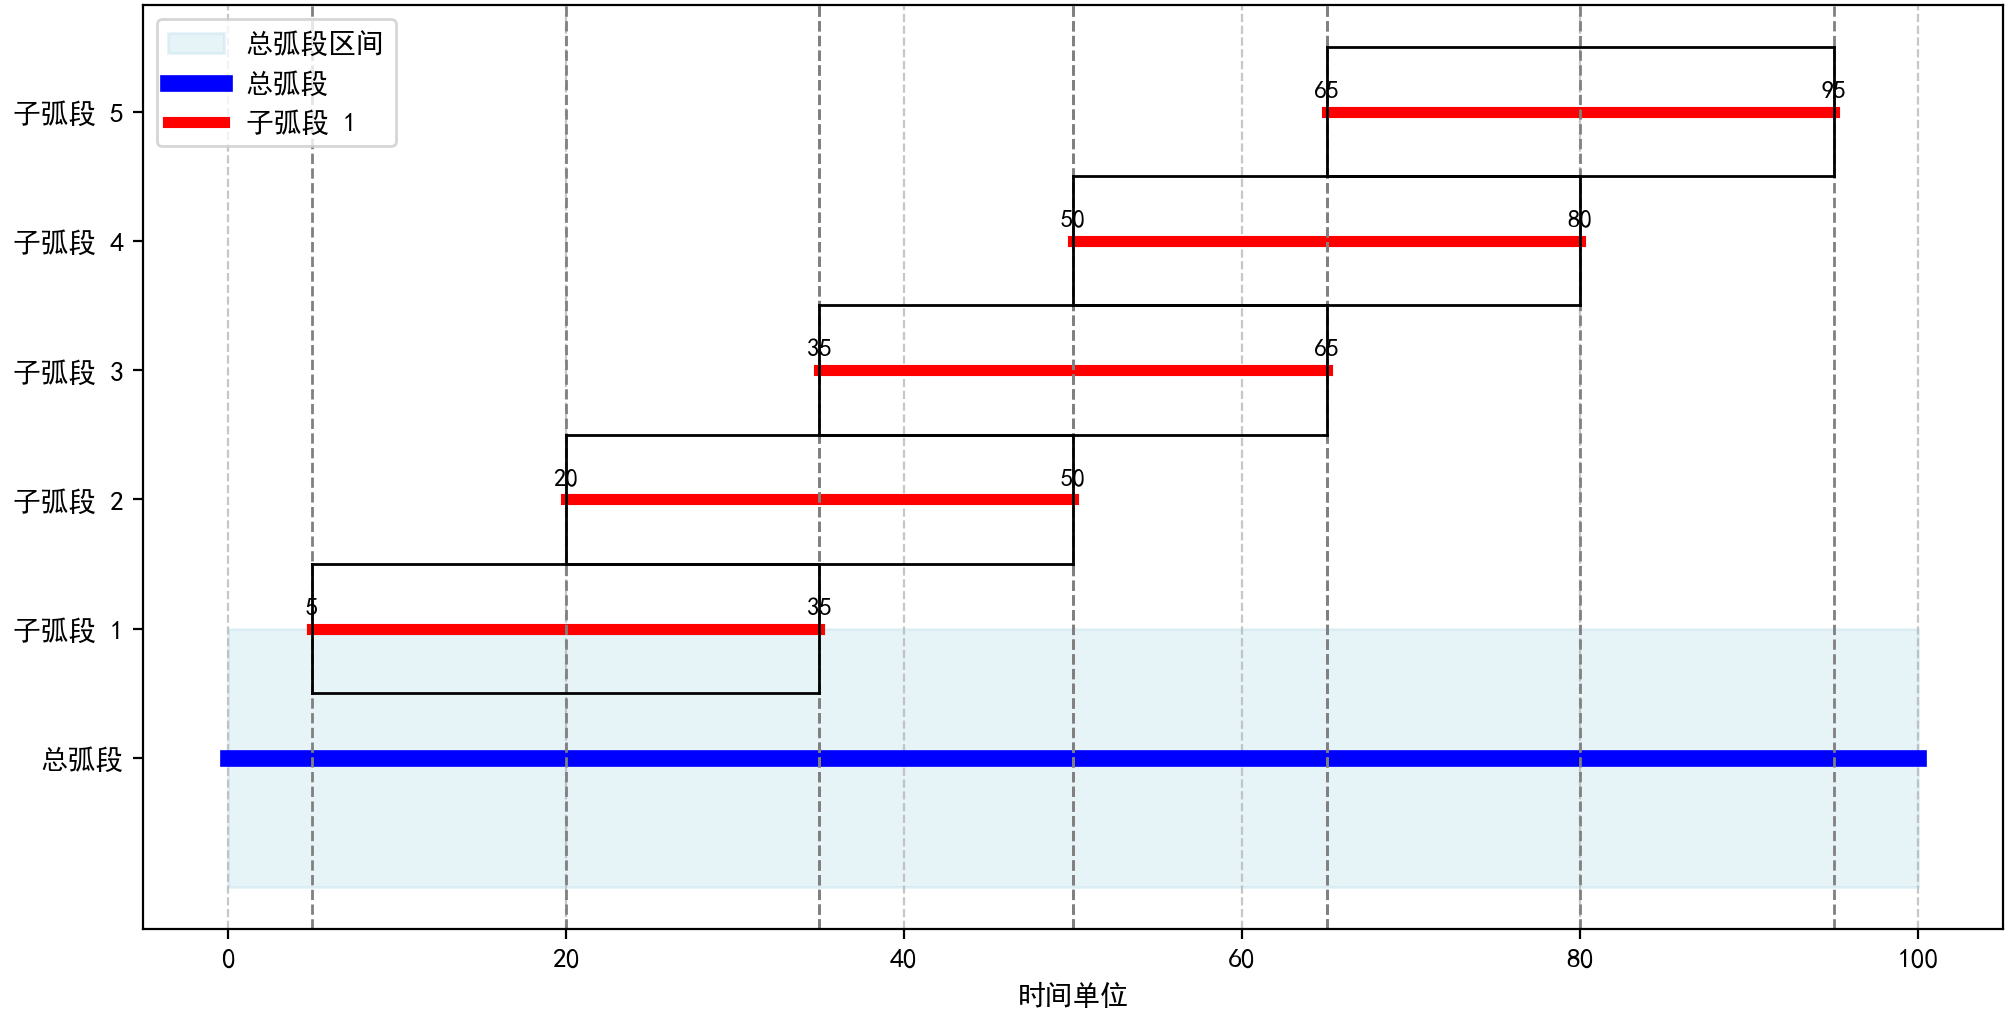
\includegraphics[width=\columnwidth]{figures/弧段切割示意图.png}
    \caption{弧段切割示意图}
    \label{fig:弧段切割示意图}
\end{figure}

切割后的子弧段需满足以下条件:  
\begin{itemize}
    \item 持续时间严格等于 $T_s^{\min}$;
    \item 起止时间索引对应仿真时间节点数组 \texttt{simDate};
    \item 若原弧段不足以生成一个完整子弧段,则保留原弧段不变。
\end{itemize}

通过此方法,系统能更好地适应多目标并发观测的需求,同时避免因弧段过长而浪费雷达资源。切割后的新弧段集合被存储在字典结构 \texttt{radar\_target\_vis\_dict} 中,并用于后续的模型构建与求解。

\subsection{问题求解流程}
问题求解流程图如\autoref{figure:问题求解流程图}所示。
\begin{figure}[h]\centering
    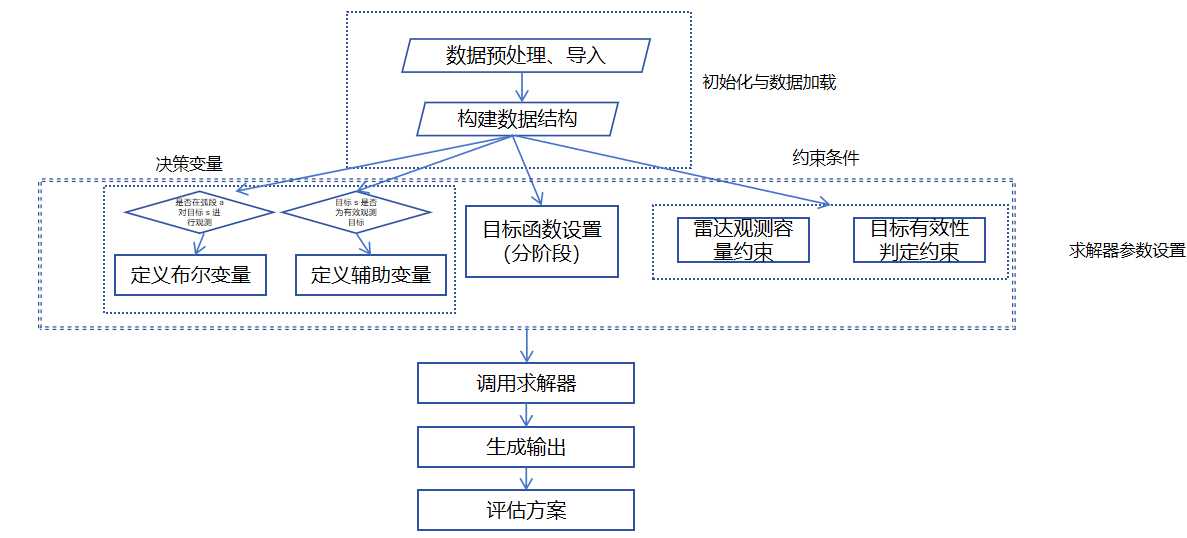
\includegraphics[width=\columnwidth]{figures/问题求解流程图.png}
    \caption{问题求解流程图}
    \label{figure:问题求解流程图}
\end{figure}

\newpage
\section{探测任务规划方法说明}
\subsection{使用的求解器}
本项目使用杉数科技提供的商业混合整数规划求解器 COPT(Cardinal Optimizer)。该求解器支持高性能求解大规模 MILP、MIQP 等优化问题,并支持 Python 接口与 Gurobi 接近。具体使用过程中,通过构建 COPT 模型对象、添加变量与约束、设置目标函数并调用 \texttt{model.solve()} 进行求解。

\subsection{规划方法的基本原理}
我们采用整数规划方法对问题建模求解。初始时,程序从观测窗口表中构建弧段数据,并根据任务参数构建布尔决策变量。每轮迭代中,求解器根据目标函数动态调整变量组合,直至收敛或达到终止条件。由于初期目标函数值往往较低,求解器通过迭代优化调度方案,逐步提升有效观测数量,提升资源利用率。在建模过程中,我们将目标函数设置为最大化加权有效观测目标数。

\subsection{程序说明}
为了便于后续阅读和理解,下面列出了主要涉及的集合、参数和变量(如\autoref{table:主要数据结构与符号说明}所示)。其中,弧段集合 $A_{r,s}$ 的生成依赖于观测窗口字典 \texttt{radar\_target\_vis\_dict}。该字典的键为测站-目标编号对 $(r,s)$,值为该测站可观测该目标的多个时间窗口,每个时间窗口用一个三元组 $(t_{\text{start}}, t_{\text{end}}, \Delta t)$ 表示,分别对应仿真起止时间点的索引与持续时长(分钟)。该结构最初由可见性分析模块根据轨道仿真生成,并经由 MATLAB 的 \texttt{usableArcs.mat} 文件导入。

变量 \texttt{x[r][s][a]} 为核心的布尔决策变量,用于表示是否选择雷达 $r$ 在第 $a$ 个弧段上观测目标 $s$。该变量由 COPT 求解器在建模阶段创建,在求解后可通过 \texttt{x[r][s][a].x} 获取其值(0 或 1)。变量 \texttt{y[s]} 表示目标 $s$ 是否被有效观测(即满足其所有观测需求约束),是模型中用于综合评估任务完成情况的辅助变量。

输入数据结构中,\texttt{sensor\_data} 与 \texttt{require\_data} 分别来自 Excel 文件 \texttt{sensorData.xlsx} 和 \texttt{requireData.xlsx},字段对应关系如\autoref{tab:data-fields}所示。
\begin{table}[H]
    \centering
    \caption{输入数据字段与模型变量的对应关系}
    \label{tab:data-fields}
    \begin{tabular}{lll}
        \toprule
        \textbf{数据字段来源}        & \textbf{字段名称}            & \textbf{模型中对应符号}      \\
        \midrule
        \texttt{sensor\_data}  & \texttt{雷达编号}            & 构建雷达集合 $R$            \\
                               & \texttt{最大探测目标数}         & 各雷达最大观测能力 $C_r$       \\
        \addlinespace
        \texttt{require\_data} & \texttt{目标编号}            & 构建目标集合 $S$            \\
                               & \texttt{需要的测站数量}         & 最小观测测站数 $M_s^{\min}$  \\
                               & \texttt{需要的弧段数量}         & 最小观测弧段数 $N_s^{\min}$  \\
                               & \texttt{需要的观测时间(min)}    & 最小累计观测时长 $T_s^{\min}$ \\
                               & \texttt{优先级(数值越大,优先级越高)} & 优先级权重 $w_s$           \\
        \bottomrule
    \end{tabular}
\end{table}

程序通过读取测站参数表 \texttt{sensorData.xlsx} 生成数据框 \texttt{sensor\_data},其中字段 \texttt{sensor\_data["雷达编号"]} 提供每个测站的唯一标识,用于构建雷达集合 $R$;字段 \texttt{sensor\_data["最大探测目标数"]} 表示每个测站在任一时刻最多可同时观测的目标数,对应模型中的参数 $C_r$。任务需求表 \texttt{requireData.xlsx} 被加载为数据框 \texttt{require\_data},记录每一个观测目标的基本属性及其观测需求:\texttt{require\_data["目标编号"]} 用于构建目标集合 $S$;\texttt{require\_data["需要的测站数量"]} 表示每个目标所需的最小观测测站数,记作 $M_s^{\min}$;\texttt{require\_data["需要的弧段数量"]} 表示所需的最小观测次数,记作 $N_s^{\min}$;\texttt{require\_data["需要的观测时间(min)"]} 是累计观测时长的最小值(单位为分钟),映射为 $T_s^{\min}$;而 \texttt{require\_data["优先级(数值越大,优先级越高)"]} 表示任务重要性,用于构建目标函数中的权重系数 $w_s$。

此外,时间节点矩阵 \texttt{simDate} 是一个二维数组,表示整个仿真周期内的统一时间参考,供弧段时间索引定位与可视化模块使用。仿真起始时间 \texttt{start\_time} 用于构造 UTC 时间标签。通过模型求解后,遍历所有 \texttt{x[r][s][a]} 的值即可输出完整的调度方案,包括观测起止时间与分配的测站资源,适用于后续的任务下发与动态更新。

\newpage
\section{探测任务方案生成结果}
\subsection{仿真参数}
\subsubsection{必做任务}
在必做仿真实验中,我们选择了 193 颗星链卫星以及 40 部地面雷达(包含精密跟踪雷达和相控阵雷达)进行调度仿真。具体参数如\autoref{table:必做任务仿真参数设置}所示。
\begin{table}[h]
    \centering
    \caption{仿真参数设置}
    \label{table:必做任务仿真参数设置}
    \begin{tabular}{>{$}l<{$} | l | l}
        \hline
        \textbf{参数名称}  & \textbf{说明} & \textbf{数值}                    \\
        \hline
        \Delta t       & 时间步长        & 1\,\text{min}                  \\
        T_{\text{sim}} & 仿真总时长       & 1440\,\text{min}(1天)           \\
        T_s^{\min}     & 各目标最小观测时长   & 3\,\text{min} -- 6\,\text{min} \\
        M_s^{\min}     & 各目标所需最小测站数量 & 2 -- 3                         \\
        N_s^{\min}     & 各目标最小有效观测次数 & 4 -- 6                         \\
        C_r            & 各雷达的同时观测容量  & 1(精密跟踪)或 80(相控阵)               \\
        \omega_s            & 各目标的优先级  & 6--10               \\
        \hline
    \end{tabular}
\end{table}
\subsubsection{选做任务}
在选做仿真实验中,我们选择了 40 部地面雷达(包含精密跟踪雷达和相控阵雷达),分别选择了 5000 颗或11113颗卫星进行调度仿真。具体参数如\autoref{table:选做任务仿真参数设置}所示。
\begin{table}[h]
    \centering
    \caption{仿真参数设置}
    \label{table:选做任务仿真参数设置}
    \begin{tabular}{>{$}l<{$} | l | l}
        \hline
        \textbf{参数名称}  & \textbf{说明} & \textbf{数值}                    \\
        \hline
        \Delta t       & 时间步长        & 1\,\text{min}                  \\
        T_{\text{sim}} & 仿真总时长       & 1440\,\text{min}(1天)           \\
        T_s^{\min}     & 各目标最小观测时长   & 3\,\text{min} -- 6\,\text{min} \\
        M_s^{\min}     & 各目标所需最小测站数量 & 2 -- 3                         \\
        N_s^{\min}     & 各目标最小有效观测次数 & 3 -- 4                         \\
        C_r            & 各雷达的同时观测容量  & 1(精密跟踪)或 80(相控阵)               \\
        \omega_s            & 各目标的优先级  & 1--5               \\
        \hline
    \end{tabular}
\end{table}
\subsection{探测任务方案结果}
在进行整数规划求解后,获得了一组可行的观测任务分配方案。\autoref{tab:schedule_summary}是必做任务的部分雷达-目标观测计划摘要。此外,我们运用HTML的形式,能够选择想要展示的方式,展示任务分配表格和任务甘特图。单个测站的甘特图如\autoref{figure:102测站分配的任务甘特图}所示。单个目标被分配的观测任务如\autoref{figure:63411目标被分配的任务甘特图}所示。HTML网页操作界面如\autoref{figure:网页界面示意}所示。
\begin{figure}[htbp]\centering
	\begin{minipage}[b]{0.49\columnwidth}\centering
		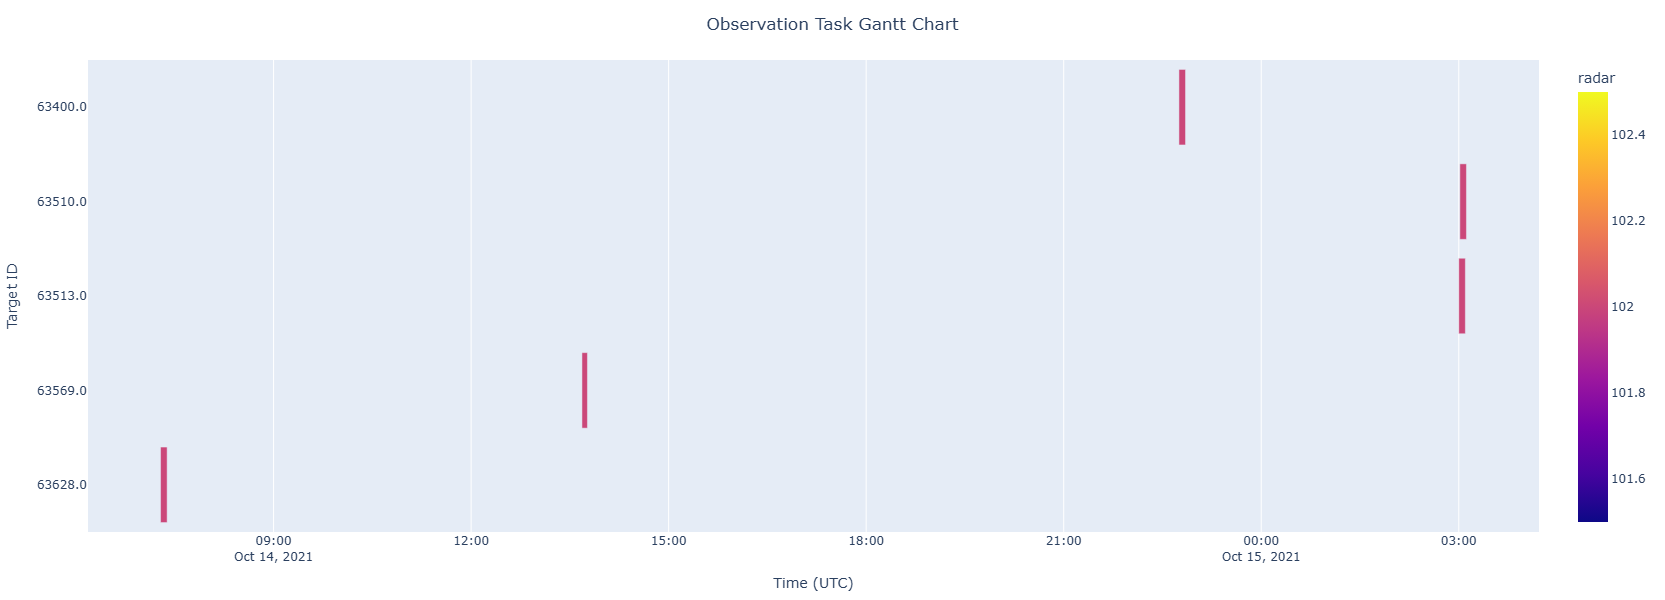
\includegraphics[width=\linewidth]{figures/102测站.png}\subcaption{102测站分配的任务甘特图}\label{figure:102测站分配的任务甘特图}
	\end{minipage}
	\begin{minipage}[b]{0.49\columnwidth}\centering
		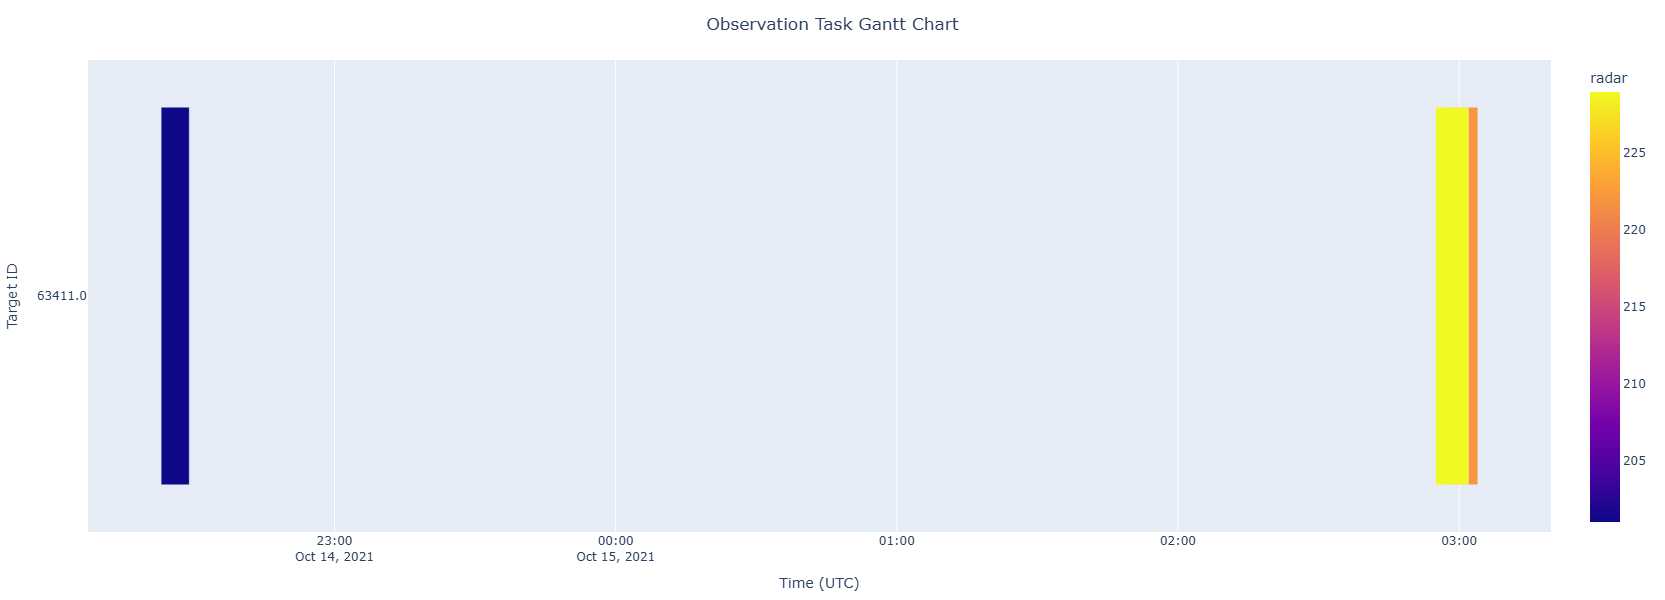
\includegraphics[width=\linewidth]{figures/63411目标.png}\subcaption{63411目标被分配的任务甘特图}\label{figure:63411目标被分配的任务甘特图}
	\end{minipage}
	\caption{网页界面示意}\label{figure:网页界面示意}
\end{figure}

三组数据都求出了最优解。
\subsubsection{必做任务}
在必做任务中,仅有188颗目标星在任务时间范围内有可用观测弧段,故至多可以覆盖188颗星。所以结果达成了100\%覆盖率。求解时间为1.22秒,变量数量为:41060个0/1型变量,386个整数变量。经过COPT求解器优化(预处理),变量数量变为:7365个0/1型变量,18个整数变量。
\begin{table}[h]
    \centering
    \caption{探测任务规划必做任务求解结果统计}
    \label{tab:探测任务规划必做任务求解结果统计}
    \begin{tabularx}{0.8\columnwidth}{Xl}
        \toprule
        \textbf{指标}        & \textbf{数值}      \\
        \midrule
        最终目标值(加权有效观测目标数)   & 1476.0           \\
        总目标数量              & 193              \\
        有效观测目标数量           & 188              \\
        覆盖率                & 97.41\%          \\
        高优先级目标覆盖率(优先级 > 8) & 63/65 → 96.92\%  \\
        中优先级目标覆盖率(优先级 > 6) & 96/99 → 96.97\%  \\
        低优先级目标覆盖率          & 29/29 → 100.00\% \\
        \bottomrule
    \end{tabularx}
\end{table}

\subsubsection{选做任务}
在5000颗卫星中,仅有4313颗目标星在任务时间范围内有可用观测弧段,故至多可以覆盖4313颗星。最终覆盖了有效目标4306个,覆盖率86.12\%。求解时间为13.89秒,变量数量为:0/1型变量988417个,整数变量10000个。经过COPT求解器优化(预处理),变量数量变为:50063个0/1型变量,244个整数变量。

在11113颗卫星中,仅有10323目标星在任务时间范围内有可用观测弧段,故至多可以覆盖10323颗星。最终覆盖了有效目标10316个,覆盖率92.83\%。求解时间为584.81秒,变量数量为:0/1型变量2338896个,整数变量22226个。经过COPT求解器优化,问题的变量数量被优化为:0/1型变量678131个,整数变量1189个。

\begin{table}[h]
    \centering
    \caption{探测任务规划选做任务1求解结果统计}
    \label{tab:探测任务规划选做任务1求解结果统计}
    \begin{tabularx}{0.8\columnwidth}{Xl}
        \toprule
        \textbf{指标}        & \textbf{数值}      \\
        \midrule
        最终目标值(加权有效观测目标数)   & 12914.0           \\
        总目标数量              & 5000              \\
        有效观测目标数量           & 4306              \\
        覆盖率                & 86.12\%          \\
        高优先级目标覆盖率(优先级 > 3) & 548/621→ 88.24\%  \\
        中优先级目标覆盖率(优先级 > 2) & 2152/2516 → 85.53\%  \\
        低优先级目标覆盖率          & 1606/1863 → 86.21\% \\
        \bottomrule
    \end{tabularx}
\end{table}

\begin{table}[h]
    \centering
    \caption{探测任务规划选做任务2求解结果统计}
    \label{tab:探测任务规划选做任务2求解结果统计}
    \begin{tabularx}{0.8\columnwidth}{Xl}
        \toprule
        \textbf{指标}        & \textbf{数值}      \\
        \midrule
        最终目标值(加权有效观测目标数)   & 30939.0           \\
        总目标数量              & 11113              \\
        有效观测目标数量           & 10316              \\
        覆盖率                & 92.83\%          \\
        高优先级目标覆盖率(优先级 > 3) & 1294/1383 -> 93.56\%  \\
        中优先级目标覆盖率(优先级 > 2) & 5150/5561 -> 92.61\%  \\
        低优先级目标覆盖率          & 3872/4169 -> 92.88\% \\
        \bottomrule
    \end{tabularx}
\end{table}

\newpage
\section{探测任务方案评估}
本节将从以下几个方面对探测任务调度方案进行评估:
\begin{itemize}
    \item {目标覆盖效果}:统计有效观测目标的数量及覆盖率,评估调度方案是否满足任务需求;
    \item {资源利用效率}:通过雷达观测弧段总数评估雷达资源的使用效率;
    \item {优先级响应程度}:按优先级统计各层级目标的覆盖率,验证模型是否合理响应优先级设定;
    \item {计算性能表现}:评估模型求解时间、收敛速度及稳定性。
\end{itemize}

评估结果如\autoref{tab:探测任务规划必做任务求解结果统计}、\autoref{tab:探测任务规划选做任务1求解结果统计}和\autoref{tab:探测任务规划选做任务2求解结果统计}所示。模型在优先保障高权重目标的前提下,仍能兼顾大量中低优先级目标的观测需求,体现了良好的任务协调能力。此外,雷达资源利用较为紧凑,观测弧段总数控制在合理范围内,表明模型具有较高的资源调度效率。

\section{拓展思考}
通过本次“探测任务规划”与前期“近距离观测轨迹规划”的仿真实践,我对航天任务规划问题有了更加深入的理解。航天任务规划本质上是一个涉及复杂资源调度与多目标优化的问题,其核心在于如何在有限的时间、设备与资源下,最大化任务收益,并确保任务的可行性。

在建模过程中,我们尝试了两阶段建模策略,但发现效率较低。经过深入分析后,我们发现问题出在约束条件的设置上。具体来说,我们原本将 \texttt{y} 变量的约束条件设置为“大于等于”形式,这使得计算过程的复杂度较高,导致了较大的资源消耗和较长的计算时间。后来,我们将约束条件修改为“等于”形式,显著提高了程序的效率,并减少了不必要的求解阶段。这个调整不仅减少了计算的复杂度,还降低了资源消耗,最终提升了整个优化过程的效率。

以下是我们在两阶段求解方法中的约束条件修改前后的主要变化说明:

3. 判断目标是否为有效观测目标:

原先的约束条件形式为:
$$
y_s = 
\begin{cases}
1, & \text{if } N_r(s) \geq M_s^{\min} \text{ and } \sum_{r \in R} \sum_{a \in A_{r,s}} x_{r,s,a} \geq N_s^{\min} \\
0, & \text{otherwise}
\end{cases}
$$
其中:
\begin{itemize}
    \item $M_s^{\min}$:目标 $s$ 所需的最小观测测站数;
    \item $N_s^{\min}$:目标 $s$ 所需的最小有效观测次数。
\end{itemize}

这个约束条件的原始形式使用了“大于等于”($\geq$)操作符,导致模型在求解时面临较大的解空间,从而增加了求解的难度和时间。在修改后,我们将“大于等于”条件改为了“等于”条件,即:
$$
y_s = 
\begin{cases}
1, & \text{if } N_r(s) = M_s^{\min} \text{ and } \sum_{r \in R} \sum_{a \in A_{r,s}} x_{r,s,a} = N_s^{\min} \\
0, & \text{otherwise}
\end{cases}
$$

通过将约束条件调整为“等于”形式,程序的解空间被有效缩小,我们也将原来设置的二阶段求解,直接简化为了一阶段求解,计算效率得到显著提高,且求解过程更加稳定。

\begin{sidewaystable}[h]
    \centering
    \caption{主要数据结构与符号说明}
    \label{table:主要数据结构与符号说明}
    \begin{tabularx}{\columnwidth}{llXl}
        \toprule
        类别   & 符号/变量                                                  & 含义                                             & 数据类型                       \\
        \midrule
        集合   & $R$ / \texttt{radars}                                  & 雷达编号集合,编号从0开始                                  & \texttt{list[int]}         \\
             & $S$ / \texttt{targets}                                 & 目标编号集合,编号从0开始                                  & \texttt{list[int]}         \\
             & $T$ / \texttt{simDate}                                 & 仿真时间节点序列(UTC)                                  & \texttt{np.ndarray[float]} \\
             & $A_{r,s}$ / \texttt{arc\_indices[(r,s)]}               & 雷达$r$对目标$s$的可用弧段编号集合                           & \texttt{dict[tuple,list]}  \\
        输入数据 & \texttt{sensor\_data}                                  & 测站参数表,包含编号、最大可观测目标数等信息                         & \texttt{DataFrame}         \\
             & \texttt{require\_data}                                 & 各目标观测需求表,包含所需测站数、观测次数、优先级等                     & \texttt{DataFrame}         \\
             & \texttt{usable\_arcs}                                  & 可见弧段原始矩阵(MATLAB格式)                             & \texttt{np.ndarray}        \\
             & \texttt{radar\_target\_vis\_dict}                      & 可见性字典:键为$(r,s)$,值为弧段列表$(start, end, duration)$ & \texttt{dict[tuple,list]}  \\
        模型参数 & $C_r$ / \texttt{radar\_capacities[r]}                  & 雷达$r$的最大同时观测能力                                 & \texttt{np.ndarray[int]}   \\
             & $M_s^{\min}$ / \texttt{required\_stations[s]}          & 目标$s$需被多少个测站观测                                 & \texttt{np.ndarray[int]}   \\
             & $N_s^{\min}$ / \texttt{required\_arc\_count[s]}        & 目标$s$需被观测的有效弧段数量                               & \texttt{np.ndarray[int]}   \\
             & $T_s^{\min}$ / \texttt{required\_observation\_time[s]} & 目标$s$需累计观测时间(分钟)                               & \texttt{np.ndarray[float]} \\
             & $w_s$ / \texttt{priority\_weights[s]}                  & 目标$s$的观测优先级权重                                  & \texttt{np.ndarray[float]} \\
        决策变量 & $x_{r,s,a}$ / \texttt{x[r][s][a]}                      & 布尔变量,表示是否在弧段$a$对目标$s$进行观测                      & \texttt{coptpy.Var}        \\
             & $y_s$ / \texttt{y[s]}                                  & 布尔变量,表示目标$s$是否被有效观测                            & \texttt{coptpy.Var}        \\
        \bottomrule
    \end{tabularx}
\end{sidewaystable}

\begin{sidewaystable}[h]
    \centering
    \caption{部分调度方案摘要(前10项)}
    \label{tab:schedule_summary}
    \begin{tabular}{|c|c|c|c|c|c|}
        \hline
        \textbf{雷达编号} & \textbf{目标编号} & \textbf{弧段索引} & \textbf{开始时间 (UTC)} & \textbf{结束时间 (UTC)} & \textbf{持续时间 (分钟)} \\
        \hline
        101.0         & 63454.0       & 2             & 2021-10-14T08:03:00 & 2021-10-14T08:08:00 & 5.0                \\
        \hline
        102.0         & 63400.0       & 2             & 2021-10-14T22:45:00 & 2021-10-14T22:51:00 & 6.0                \\
        \hline
        102.0         & 63510.0       & 1             & 2021-10-15T03:01:00 & 2021-10-15T03:07:00 & 6.0                \\
        \hline
        102.0         & 63513.0       & 2             & 2021-10-15T03:00:00 & 2021-10-15T03:06:00 & 6.0                \\
        \hline
        102.0         & 63569.0       & 0             & 2021-10-14T13:41:00 & 2021-10-14T13:46:00 & 5.0                \\
        \hline
        102.0         & 63628.0       & 0             & 2021-10-14T07:17:00 & 2021-10-14T07:23:00 & 6.0                \\
        \hline
        108.0         & 63401.0       & 4             & 2021-10-15T03:37:00 & 2021-10-15T03:42:00 & 5.0                \\
        \hline
        108.0         & 63453.0       & 4             & 2021-10-14T13:01:00 & 2021-10-14T13:05:00 & 4.0                \\
        \hline
        108.0         & 63454.0       & 0             & 2021-10-14T04:44:00 & 2021-10-14T04:49:00 & 5.0                \\
        \hline
        108.0         & 63594.0       & 2             & 2021-10-14T18:15:00 & 2021-10-14T18:19:00 & 4.0                \\
        \hline
    \end{tabular}
\end{sidewaystable}

\newpage
\section*{A.1 数据模块}
\lstinputlisting[language=Python,caption={数据模块}]{../data.py}

\newpage
\section*{A.2 数据处理模块}
\lstinputlisting[language=Python,caption={数据处理模块}]{../data_processing_module.py}

\newpage
\section*{A.3 结果展示模块}
\lstinputlisting[language=Python,caption={结果展示模块}]{../result_show_app.py}

\end{document}